\apendice{Documentación técnica de programación}

\section{Introducción}
En este apartado se incluye la información técnica relacionada con la acometida y con el código, incluyendo la estructura de directorios y todo el proceso de instalación física así como los pasos necesarios para la obtención de los diferentes tokens.

\section{Estructura de directorios}
Para comprender la estructura de directorios debemos conocer las diferentes partes del proyecto y tener en cuenta que son completamente diferentes, aunque en este proyecto se han integrado para poder hacer uso del sistema domótico. 

Tras accederal directorio raiz del proyecto vemos dos directorios, \textbf{credentials} y \textbf{source}. Dentro de \textbf{credentials} tenemos el archivo principal de configuración y dentro de \textbf{source} el resto de directorios del proyecto. Nada más acceder al directorio \textbf{source} podemos ver tres directorios principales:

\begin{figure}[h]
\centering
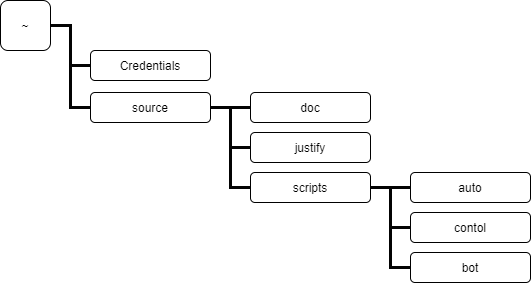
\includegraphics[width=0.9\textwidth]{img/Diagramas/directorios1.png}
\caption{Árbol de directorios.}\label{Directorios}
\end{figure}

\begin{enumerate}
    \item El directorio~\textbf{doc} contiene la redacción del proyecto.
    \item El directorio~\textbf{justify} contiene las normativas aplicables en la instalación física.
    \item El directorio~\textbf{scripts} es el que contiene todo el código del proyecto.
\end{enumerate}

Para entender la organización del directorio que almacena el código hay que saber que el código se divide, principalmente, en tres partes, que podemos verlas en la figura~\ref{SecAcSys} son las siguientes:

\begin{itemize}
    \item La parte de toma de datos.
    \item La parte de mensajería.
    \item La parte física de nuestra instalación domótica, incluyendo la Raspberry Pi.
\end{itemize}


Por ello, dentro del directorio llamado <<scripts>> que es el que almacena nuestro código, éste se ha estructurado en tres partes:
\begin{itemize}
    \item La carpeta \textbf{auto}, que permite obtener la información de las APIs seleccionadas de Internet.
    \item La carpeta \textbf{bot}, donde almacenamos la configuración de nuestro bot.
    \item La carpeta \textbf{control}, donde almacenamos los scripts de control de la instalación domótica.
\end{itemize}

En todas ellas, los scripts, tanto de Bash como de Python llevan la cabecera específica para el tipo de código contenido en el archivo:

\begin{lstlisting}[language=python,firstnumber=0, basicstyle=\normalsize]
#!/usr/bin/env python3
\end{lstlisting}

Ésta es la cabecera para los archivos Bash:
\begin{lstlisting}[language=sh,firstnumber=0, basicstyle=\normalsize]
#!/bin/bash
\end{lstlisting}

He introducido estas cabeceras porque, sin ellas, he tenido problemas al lanzar las instrucciones desde otro script.

\subsection{Carpeta auto}
Al comienzo del proyecto esperé encontrar alguna web desde la que poder recoger la información haciendo webscraping pero tras valorarlo detenidamente en las tutorías me decanté por el uso de APIs. Uno de los motivos es que una web es más susceptible de sufrir cambios que una API que se ha predispuesto para una función específica. Finalmente, dispuse el proyecto para poder funcionar con dos APIs públicas y gratuitas para dotar a nuestro sistema domótico de autonomía.

Las siguientes fases de la parte de toma de datos, se albergan en la carpeta auto ya que es un proceso automatizado que permite al sistema obtener los datos de forma desatendida y continua.
El proceso de automatización comprende varias fases:
\begin{enumerate}
    \item La fase de~\textbf{recopilación} de datos.
    \item La fase de~\textbf{lectura} local de parámetros.
    \item El~\textbf{cocinado} de los datos.
    \item El~\textbf{grabado} de datos en el sistema local.
\end{enumerate}
La fase de~\textbf{recopilación} de datos llama a la API de~\textbf{geolocalización} y nos devuelve, entre otros, los parámetros de nuestra ubicación en formato de latitud y longitud. Posteriormente, estos datos de ubicación son necesarios para incorporarlos en la consulta de las APIs de~\textbf{meteorología} y~\textbf{astronomía} y obtener la información de la salida y puesta del sol así como la información de las temperaturas del día siguiente en dicha ubicación. Con esta recopilación de datos tenemos la base para poder determinar el comportamiento autónomo que necesitamos por lo que almacenaremos esta información en un archivo de datos.

El siguiente paso es leer las preferencias del usuario, que se almacenan en el archivo de condicionantes. Y, una vez tengamos estos datos, podemos pasar a generar el Cron para controlar de forma automática toda la instalación y generar el diagrama de temperaturas para poder enviarlo cuando se solicite. Las imágenes se almacenan dentro del directorio ./diagramas, en formato PNG.

Estas fases se han confeccionado al final del proyecto puesto que al principio se desarrolló de forma unitaria pero surgió el problema de que, cada vez que queríamos hacer una modificación en el sistema domótico de cualquier índole, teníamos que hacer una petición nueva a las APIs y generar de nuevo un archivo Cron con los parámetros del usuario <<al vuelo>> para conseguir regenerar la automatización con los parámetros nuevos. Este sistema funcionaba correctamente pero era poco eficiente puesto que se multiplican las operaciones en función de las veces que se quiera modificar algún parámetro.
Únicamente he permitido realizar dos salidas <<al vuelo>> tras obtener los datos, estos son: el grabado de los datos recién obtenidos y la gráfica de las temperaturas conforme a dichos datos.

He tenido algunos problemas al realizar varias peticiones a las APIS ya que, por falta de permisos, no podía sobreescribir los archivos ni las imágenes. Para subsanarlo, incluí una restricción para modificar los permisos de los archivos de forma que únicamente pueden acceder el propietario y el grupo.

\subsection{Carpeta control}
La carpeta control alberga aquellos scripts bash que controlan los periféricos. Este punto únicamente me dio problemas a la hora de implantarlo desde el bot, que se subsanó con la librería os.

\subsection{Carpeta bot}
La carpeta bot contiene varios archivos, desde el archivo de control del bot hasta otros que contienen la mayoría de funcionalidades de éste. En primera instancia, se dispuso todo el código dentro del archivo de control del bot, pero por legibilidad y facilidad de mantenimiento se extrajeron las funciones.
En este punto, lo que más problemas me ha dado han sido los teclados. Como el comportamiento de los teclados es diferente entre ellos tendría que dividir las opciones del bot entre dos tipos de teclados diferentes. Finalmente, opté por no incluir estos teclados ya que no aporta funcionalidad alguna y disminuirían la legibilidad y facilidad de uso del bot. Además, para aumentar la usabilidad del bot, se ha dispuesto un menú que podemos ver al introducir el carácter <</>> además de la posibilidad de utilizar la primera letra del comando siempre que no tengamos que acompañarlo de parámetros.


\subsection{Regeneración del código al fraccionarlo por funcionalidades}

Tuve un problema en la fase de regeneración del código al fracccionarlo por funcionalidades puesto que obtenía las rutas a los archivos que necesitaba llamar de forma unitaria desde el archivo en ejecución.  Lo subsané con el siguiente código Python:
\begin{lstlisting}[language=python, firstnumber=0, basicstyle=\small]
#!/usr/bin/env python3
#Calculamos ruta
ruta=os.getcwd().split('/')
\end{lstlisting}

Tuve que realizar un paso similar para los archivos Bash:
\begin{lstlisting}[language=sh, firstnumber=0, basicstyle=\small]
#!/bin/bash
path=$(pwd)
\end{lstlisting}
Aunque en la segunda versión de código se utiliza desde la propia variable de sistema:

\begin{lstlisting}[language=sh, firstnumber=0, basicstyle=\small]
python3 ${PWD%/*}/auto/1_recabaInfo.py
python3 ${PWD%/*}/auto/3_cocinado.py
sh ${PWD%/*}/auto/4_reescribeCron.sh
\end{lstlisting}

\section{Manual del programador}
Este punto tiene como objetivo explicar los medios necesarios para continuar con el desarrollo del código así como la explicación de las partes del proyecto.
Como la parte de desarrollo se ha generado desde Raspbian OS utilizando la interfaz para desarrollo Python, <<Thonny Python IDE>>, este punto será corto ya que el propio sistema operativo dispone del software necesario.

\subsection{Requerimientos}
Para poder hacer funcionar correctamente el código se debe clonar el repositorio e instalar los <<requeriments>> que están dentro de la ruta \textbf{/source/scripts/control/}:
\begin{lstlisting}[language=sh, firstnumber=0, basicstyle=\normalsize]
pip install -r requirements
\end{lstlisting}~\\

El software necesario es:
\begin{itemize}
    \item pyTelegramBotAPI
    \item python-telegram-bot
    \item pycurl
    \item telegram
    \item urllib3
    \item simplejson
    \item datetime
    \item requests
    \item datetime
    \item pandas
    \item matplotlib
    \item bs4
\end{itemize}

También hay que generar el archivo de configuración al mismo nivel que nuestro directorio raíz, dentro de un directorio llamado <<\textbf{credentials}>>, llamado \texttt{config2.bot}, de forma que quede como en la imagen~\ref{Directorios}. La información que debe contener el archivo es la que figura en el código del listing~\ref{Config2.bot}, incluyendo los tokens correspondientes y los elementos a controlar.
En las <<releases>> ya se incorpora el directorio y una plantilla para rellenar el archivo \texttt{config2.bot} correctamente.

\subsection{Archivos}
Dentro del directorio \texttt{auto} encontramos:
\begin{itemize}
    \item \texttt{~/source/scripts/auto/1\_recabaInfo.py}: Obtiene la información necesaria de las APIS.
    \item \texttt{~/source/scripts/auto/2\_condicionantes.py}: Contiene preferencias de usuario.
    \item \texttt{~/source/scripts/auto/3\_cocinado.py}: Genera el archivo preliminar del Cron para controlar las instalaciones.
    \item \texttt{~/source/scripts/auto/4\_reescribeCron.sh}: Reescribe el archivo de configuración del servicio Cron y lo reinicia.
    \item \texttt{~/source/scripts/auto/cabecera.txt}: Contiene la cabecera que utilizamos para incluirla en Cron.
    \item \texttt{~/source/scripts/auto/CronPruebas}: Contiene el texto que se volcará al archivo de configuración de Cron.
    \item \texttt{~/source/scripts/auto/InfoRecabada}: Contiene la información que se ha obtenido de las APIs.
    \item \texttt{~/source/scripts/auto/LanzaTodoElProceso.sh}: Lanza los 4 primeros scripts de forma desatendida.
    \item \texttt{~/source/scripts/auto/log.cron}: Contiene información a consultar por el bot.
    \item \texttt{~/source/scripts/auto/obtencionDatos.py}: Nos permite leer el archivo ~/credentials.config2.bot y obtiene las rutas que utilizaremos.
\end{itemize}

Dentro del directorio \texttt{bot} encontramos:
\begin{itemize}
    \item \texttt{~/source/scripts/bot/bot.py}: Contiene el archivo de configuración del bot.
    \item \texttt{~/source/scripts/bot/datos.py}: Obtiene las horas de amanecer, anochecer, encendido de luces y subida de persianas por la mañana y los envía al usuario que lo solicita.
    \item \texttt{~/source/scripts/bot/diagramaTemperaturas.py}: Envía la última imagen generada por el sistema u otra que especifique el usuario.
    \item \texttt{~/source/scripts/bot/generador.py}: Lanza todo el proceso automático desde ./auto/LanzaTodoElProceso.sh.
    \item \texttt{~/source/scripts/bot/horaSubida.py}: Envía la hora a la que se subirán las persianas por la mañana y permite cambiarla si el usuario especifica otra hora siempre que ésta sea después de la hora de amanecer.
    \item \texttt{~/source/scripts/bot/info.py}: Nos muestra información de la máquina Raspberry Pi que soporta el Sistema.
    \item \texttt{~/source/scripts/bot/obtencionDatos.py}: Nos permite leer el archivo ~/credentials.config2.bot y obtiene las rutas que utilizaremos.
    \item \texttt{~/source/scripts/bot/subirPararBajar.py}: Nos permite controlar el movimiento de las persianas si existen en el archivo de configuración.
    \item \texttt{~/source/scripts/bot/temperaturaCalefaccion.py}: Envía la temperatura a la que queremos que se encienda la caldera y nos permite modificarla.
    \item \texttt{~/source/scripts/bot/temperaturasManana.py}: Envía la relación de temperaturas por horas en la ubicación de la máquina.
\end{itemize}

Dentro del directorio \texttt{control} encontramos:
\begin{itemize}
    \item \texttt{~/source/scripts/control/EncenderCaldera.sh}: Enciende la caldera.
    \item \texttt{~/source/scripts/control/ApagarCaldera.sh}: Apaga la caldera.
    \item \texttt{~/source/scripts/control/EstadoGPIO.sh}: Permite conocer el estado de los GPIO en ese instante de tiempo.
    \item \texttt{~/source/scripts/control/Bajar.sh}: Baja todas las persianas.
    \item \texttt{~/source/scripts/control/EstadoGPIO.sh}: Inhabilita los GPIO seleccionados.
    \item \texttt{~/source/scripts/control/LucesOff.sh}: Apaga las luces.
    \item \texttt{~/source/scripts/control/LucesOn.sh}: Enciende las luces.
    \item \texttt{~/source/scripts/control/Prueba\_General.sh}: Permite hacer una prueba de las persianas conectadas.
    \item \texttt{~/source/scripts/control/Reinicia\_Servicio\_Cron.sh}: Reinicia el servicio Cron.
    \item \texttt{~/source/scripts/control/subir.sh}: Sube todas las persianas.
    
\end{itemize}


\subsection{Configuración del bot como servicio}
El bot se puede lanzar como si fuera un script más pero en este caso es necesario incorporarlo como servicio. Esta decisión tiene beneficios, como la posibilidad de que se inicie con el sistema o que podamos lanzarlo o pararlo desde cualquier ubicación del SO sin tener que recordar la ubicación con la sentencia al efecto de <<\texttt{sudo service bot start/stop}>>. Pero, una vez que el demonio está corriendo, tenemos que tener en cuenta de que ya está levantada la instancia del bot, por lo que tendremos que detenerla a la hora de hacer algún tipo de modificación así como recordar que debemos levantarlo una vez terminemos. Los pasos a seguir están en un archivo dentro de \textbf{\textasciitilde/source/scripts/auto/}.

\section{Compilación, instalación y ejecución del proyecto}
Para realizar modificaciones en el código únicamente hay que seguir los siguientes pasos:
\begin{enumerate}
    \item Descargar la última release que exista en el repositorio de GitHub en el formato que se prefiera:~\url{https://github.com/davidelinformatico/TFG/releases}
    \item Para extraer del archivo .tar utilizar:~\\ \texttt{tar -xvf SistemaDomoticoInteligente\_v1.0.tar}.
    \item Para extraer del archivo .tar.gz utilizar:~\\ \texttt{tar xzvf SistemaDomoticoInteligente\_v1.0.tar.gz}.
\end{enumerate}
En este punto ya tendremos todos los archivos extraídos y podremos editarlos. Recordar que para completar el software hay que instalar el software especificado en el archivo \texttt{requeriments} que se realiza de forma automática al correr el archivo setup contenido en \textbf{\textasciitilde/source/scripts/auto/}. 

Hay que tener en cuenta que en este punto no existen los archivos esperados de control de periféricos, en el directorio \textbf{control} porque se generan a medida del sistema que se configure el sistema tras completar el archivo \texttt{config2.bot} por lo que también se puede modificar la creación de estos achivos.

No hace falta un software específico para poder modificar el código ya que podemos utilizar los propios de la Raspberry Pi o algún editor sencillo como Nano según nuestras preferencias.

Si el objetivo es correr el software correctamente hay que recordar que es indispensable que el archivo config2.bot esté completo y que se lance el setup contenido en \textbf{\textasciitilde/source/scripts/auto/}.

Finalmente, el proyecto puede lanzarse corriendo el archivo de configuración del bot:~\texttt{bot.py} desde un terminal sh, aunque si se precisa también se pueden lanzar los scripts del directorio~\textbf{auto} o~\textbf{control} por separado ya que, aunque funciona todo como un conjunto, podemos probarlos de forma unitaria.

\section{Pruebas del sistema}
Como el proyecto no cuenta con testigos de cambios de estado de los periféricos es imposible realizar pruebas en este punto y lo mismo sucede con la parte de domótica automatizada, es imposible determinar si un código realiza correctamente una acción física ya que aunque el código funcione correctamente puede que no se esté llevando a cabo correctamente la acción.

Por otro lado, las pruebas sobre la parte del proyecto que se comunica con las APIs y procesa la información se ha realizado de forma manual ya que únicamente son dos archivos y son relativamente cortos. 


